\documentclass{standalone}
\usepackage{amsmath}
\usepackage{tikz}
\usetikzlibrary{arrows,shapes}

% Define block styles
\tikzstyle{decision} = [ellipse, draw, text width=7em, text badly centered, inner sep=2pt]
\tikzstyle{block} = [rectangle, draw, text width=5em, text badly centered, rounded corners, minimum height=4em]
\tikzstyle{line} = [draw, -latex']

\newcommand{\bn}{\mathbf{n}}
\newcommand{\bq}{\mathbf{q}}

% compile with pdflatex, then run
% convert -density 300 enthalpy-basal-bc.pdf -quality 90 enthalpy-basal-bc.png

\begin{document}
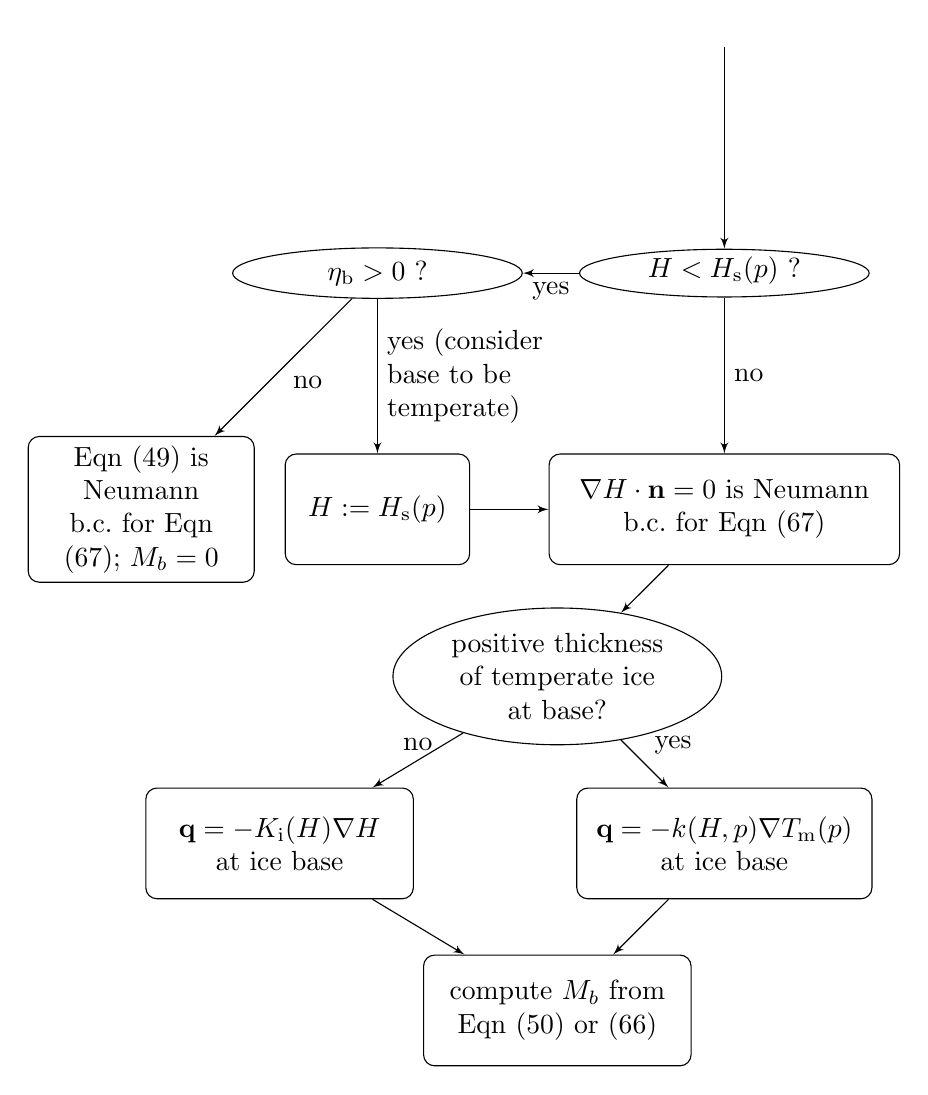
\begin{tikzpicture}[node distance = 3cm, auto]
    % Place nodes
    \node (invisiblestart) {};

    \node [decision, below of=invisiblestart, text height=0.2cm] (coldvstemp) {$H<H_{\text s}(p)$ ?};
    \node [decision, left of=coldvstemp, xshift=-4em] (excludebad) {$\eta_{\text b}>0$ ?};
    \node [block, below of=excludebad, text width=6em] (fixbad) {$H := H_{\text s}(p)$};

    % edges
    \path [line] (invisiblestart) -- (coldvstemp);
    \path [line] (excludebad) -- node [text width=6em] {yes (consider base to be temperate)} (fixbad);

    % cold branch:
    \node [block, left of=fixbad, text width=7.5em] (coldmodeltype) {Eqn (49) is Neumann b.c.~for Eqn (67); $M_b=0$};
    % edges
    \path [line] (coldvstemp) -- node {yes} (excludebad);
    \path [line] (excludebad) -- node {no} (coldmodeltype);

    % temperate branch
    \node [block, below of=coldvstemp, text width=12em] (qtemperate) {$\nabla H \cdot \bn=0$ is Neumann b.c.~for Eqn (67)};
    \node [decision, below left of=qtemperate, text width=8em] (tempthick) {positive thickness of temperate ice at base?};
    \node [block, below right of=tempthick, text width=10em] (Mbforqtemperate) {$\bq = - k(H,p)\nabla T_{\text m}(p)$ \\ at ice base};
    \node [block, below left of=tempthick, text width=9em, xshift=-4em] (Mbforqcold) {$\bq = - K_{\text i}(H) \nabla H$ \\ at ice base};
    \node [block, below left of=Mbforqtemperate, text width=9em] (getMbtemp) {compute $M_b$ from Eqn (50) or (66)};

    % edges
    \path [line] (fixbad) -- (qtemperate);
    \path [line] (coldvstemp) -- node {no} (qtemperate);
    \path [line] (tempthick) -- node [above] {no} (Mbforqcold);
    \path [line] (tempthick) -- node {yes} (Mbforqtemperate);
    \path [line] (qtemperate) -- (tempthick);
    \path [line] (Mbforqcold) -- node {} (getMbtemp);
    \path [line] (Mbforqtemperate) -- node {} (getMbtemp);
\end{tikzpicture}
\end{document}